\documentclass[11pt,a4j,dvipdfmx]{jreport}

\usepackage{comment}
\usepackage{float}
\usepackage{color}
\usepackage{multicol}
\usepackage{multirow}
\usepackage[dvipdfmx]{pict2e}
\usepackage{wrapfig}
\usepackage{graphicx}
\usepackage{bm}
\usepackage{url}
\usepackage{underscore}
\usepackage{colortbl}
\usepackage{tabularx}
\usepackage{fancyhdr}
\usepackage{ulem}
\usepackage{cite}
\usepackage{amsmath,amssymb,amsfonts}
\usepackage{algorithmic}
\usepackage{textcomp}
\usepackage{xcolor}
\usepackage[ipaex]{pxchfon}
\usepackage{pdfpages}
\usepackage{subcaption}
\usepackage{array}
\usepackage{adjustbox}
\usepackage{lipsum}

\usepackage[number-unit-product=~]{siunitx}

\usepackage[top=30truemm,bottom=30truemm,left=25truemm,right=25truemm]{geometry}

\renewcommand{\arraystretch}{1.2}

\begin{document}

\chapter{演奏実験の資料}
  被験者実験に用いた資料を以下に示す。
  \begin{quote}
    \begin{enumerate}
      \item フェイスシート
      \item アンケート用紙
      \item 研究参加同意書
      \item 演奏実験使用楽譜
      \item 演奏実験教示資料
    \end{enumerate}
  \end{quote}
  \clearpage

  \fancyhead[L]{1. フェイスシート}
  \includepdf[pages={5}, noautoscale=true, scale=0.8, pagecommand={}]{./pdfs/questions.pdf}
  \clearpage

  \fancyhead[L]{2. アンケート用紙}
  \includepdf[pages={6-16}, noautoscale=true, scale=0.8, pagecommand={}]{./pdfs/questions.pdf}
  \clearpage

  \fancyhead[L]{3. 研究参加同意書}
  \includepdf[pages={2-3}, noautoscale=true, scale=0.8, pagecommand={}]{./pdfs/questions.pdf}
  \clearpage

  \fancyhead[L]{4. 演奏実験使用楽譜}
  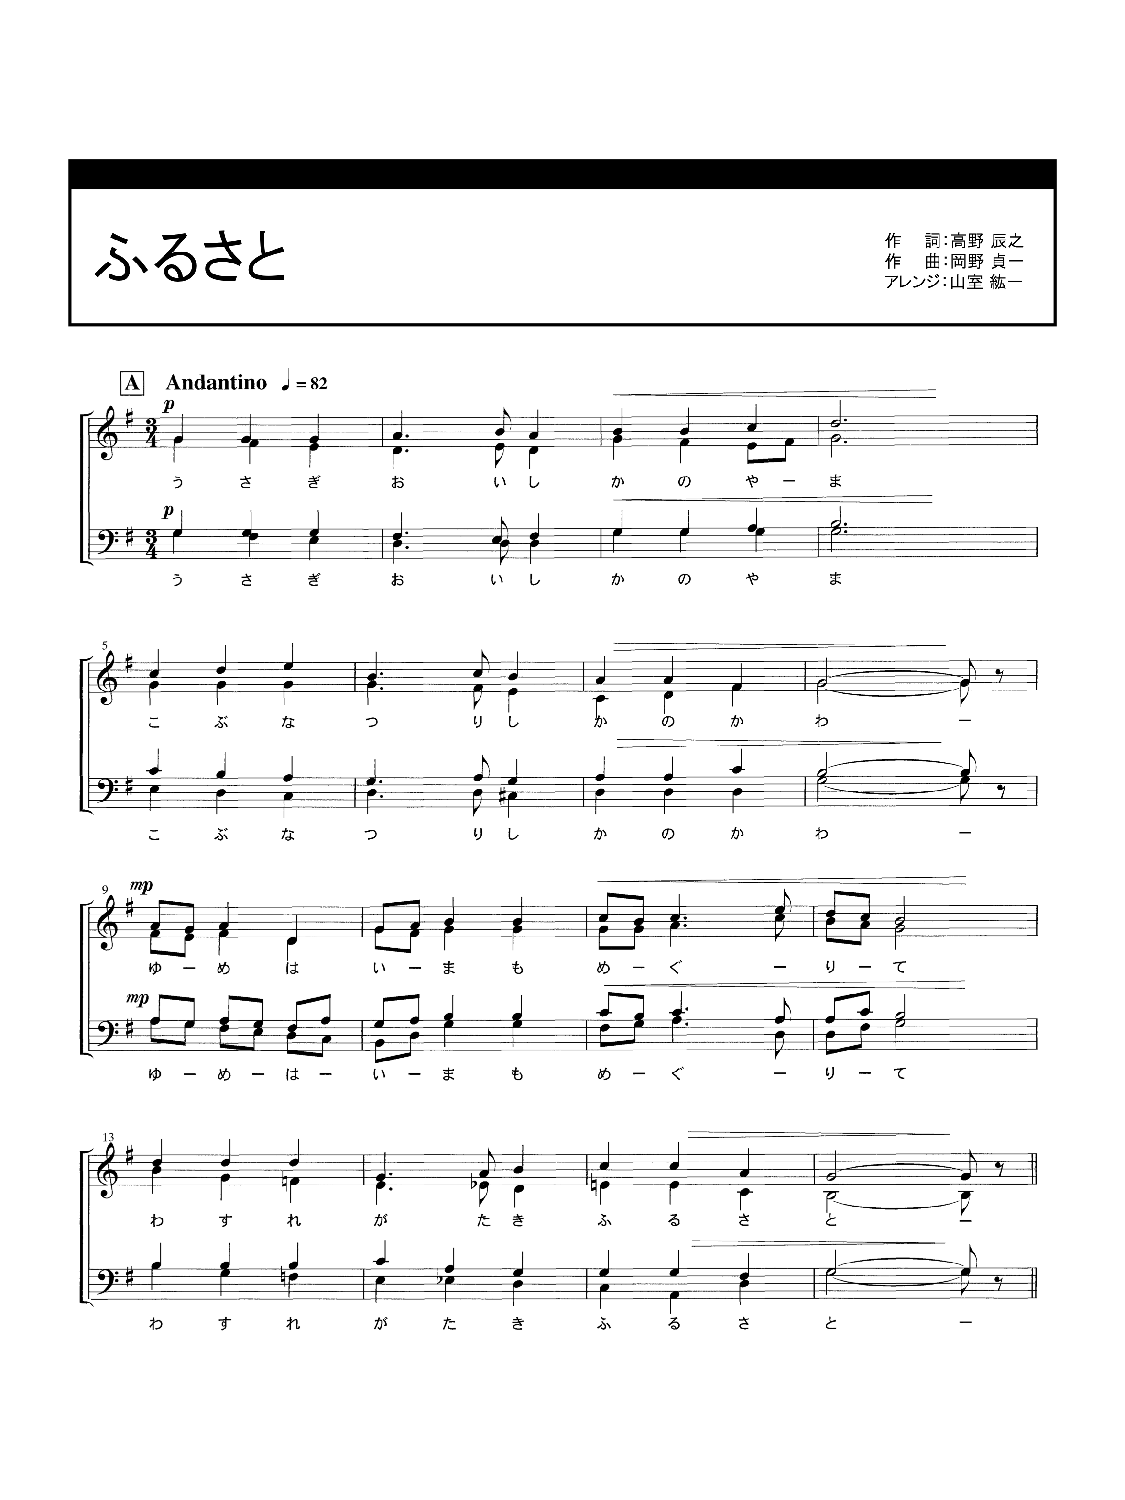
\includepdf[pages={-}, noautoscale=true, scale=0.8, pagecommand={}]{./pdfs/score.pdf}
  \clearpage

  \fancyhead[L]{5. 演奏実験教示資料}
  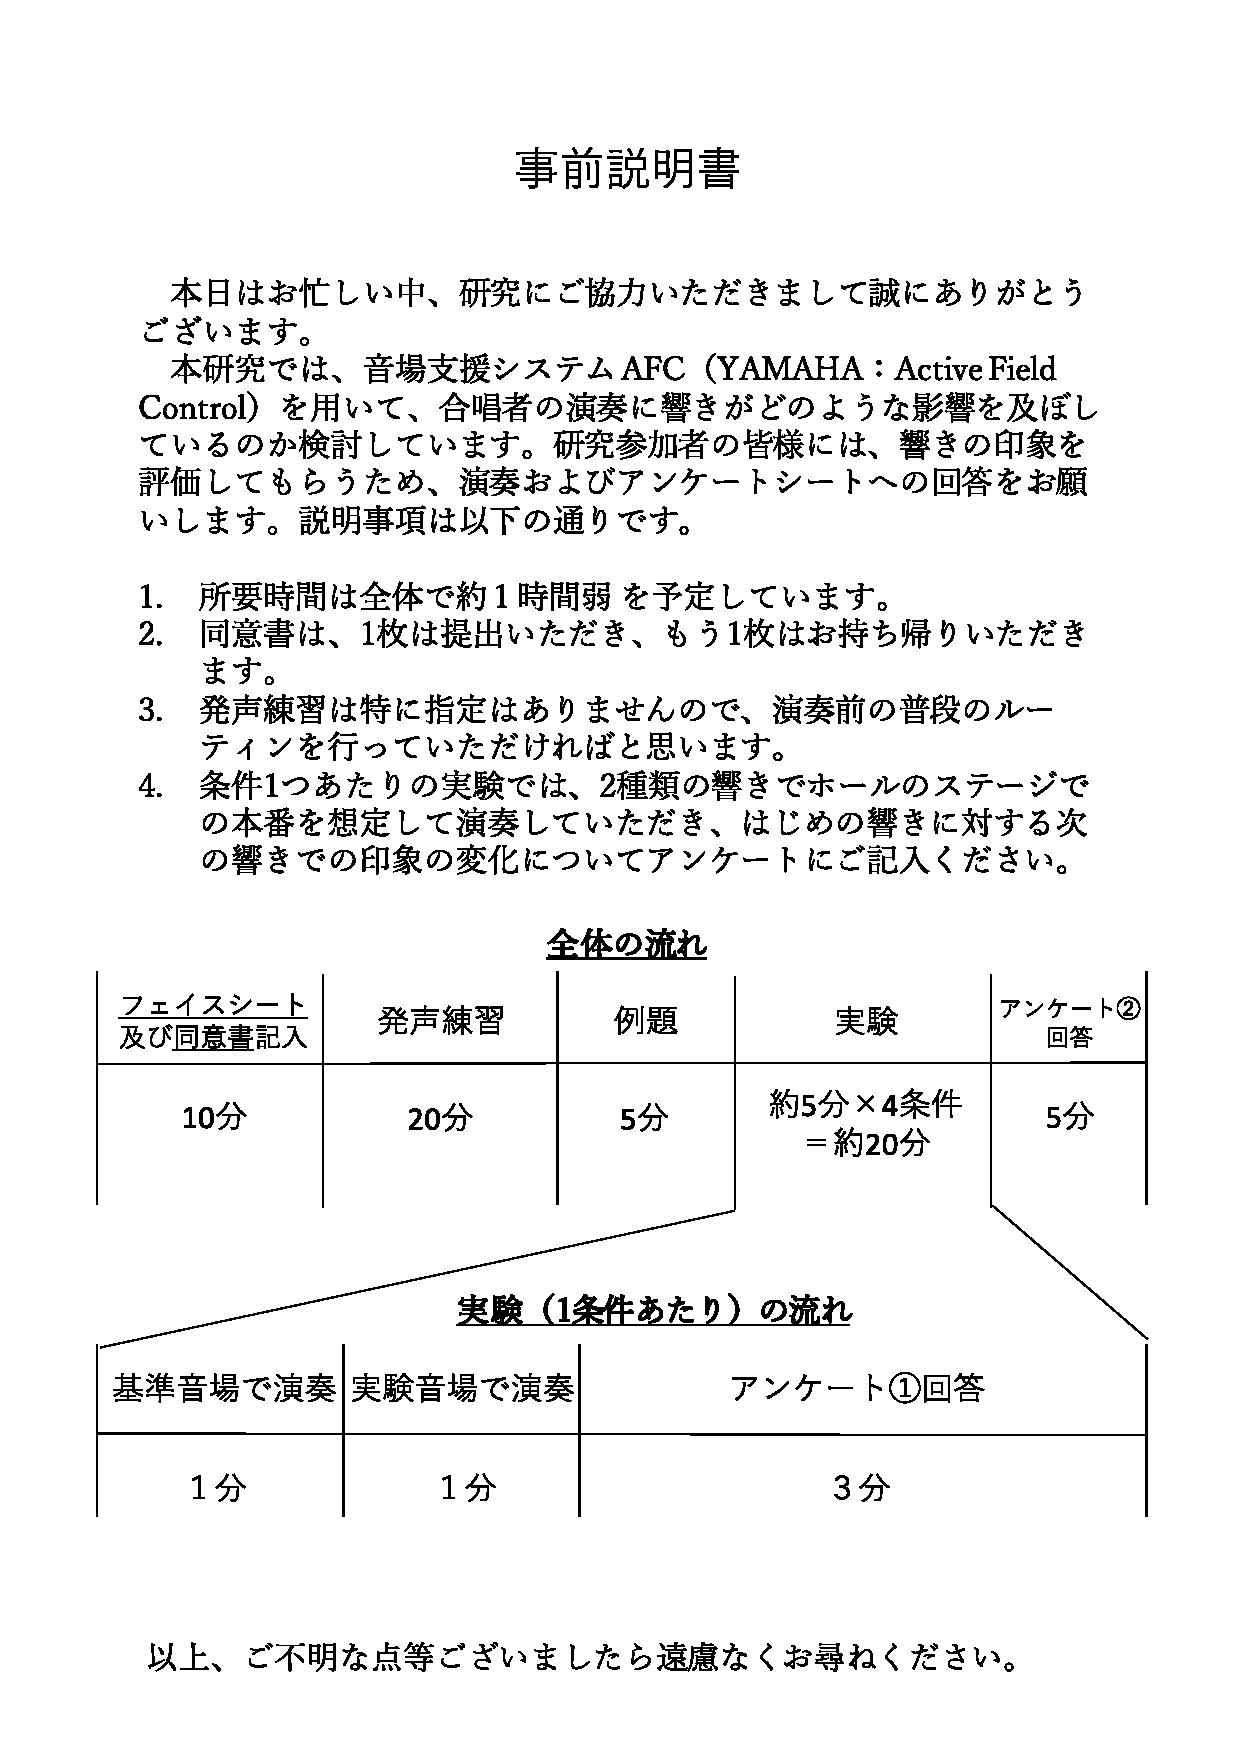
\includepdf[pages={1}, noautoscale=true, scale=0.8, pagecommand={}]{./pdfs/questions.pdf}
  \clearpage

% 参考文献
% 参考文献の箇所にインプットしてください。

% 分割ファイル内でのみ,bibliographyを読み込みます。

\expandafter\ifx\csname ifdraft\endcsname\relax

  % bibliographyを展開する

  \bibliographystyle{junsrt}
  \bibliography{ref.bib}% 同じディレクトリ内のbibファイルのみを参照可能

\fi

\end{document}